
%(BEGIN_QUESTION)
% Copyright 2011, Tony R. Kuphaldt, released under the Creative Commons Attribution License (v 1.0)
% This means you may do almost anything with this work of mine, so long as you give me proper credit

Suppose this solenoid-controlled valve refuses to open when the operator pushes the ``open'' switch:

$$\includegraphics[width=15.5cm]{i03236x01.eps}$$

You measure 0 volts AC between terminals {\bf C} and {\bf D} on the terminal strip, and then switching your multimeter to ``resistance'' you read a few ohms of resistance between the same two terminals.

A fellow technician hypothesizes that fuse F3 is blown (explaining the lack of AC voltage) {\it and} that the ``open'' pushbutton is failed-shorted (thus accounting for the low resistance measurement).  After some thought, you disagree.  You say it is more likely that either fuse F1 {\it or} F2 has blown.

\vskip 10pt

Explain why the latter hypothesis is more probable than the former, based on what you know about probability and how it relates to component failures.

\vskip 20pt \vbox{\hrule \hbox{\strut \vrule{} {\bf Suggestions for Socratic discussion} \vrule} \hrule}

\begin{itemize}
\item{} Normally one should never attempt a resistance measurement in a ``live'' electric circuit.  Explain why this is, and also why it was okay to do it here.
\item{} Suppose the failure probabilities of F1 (open), F2 (open), F3 (open), and the ``open'' pushbutton (short) are each 0.1.  Calculate the probability of either F1 or F2 failing, versus F3 and the pushbutton failing.
\end{itemize}

\underbar{file i03236}
%(END_QUESTION)





%(BEGIN_ANSWER)

This is a good example of {\it Occam's Razor}: that the best hypothesis is the one making the fewest (or the greatest-probability) assumptions.  If we assume equal PFD for each fuse, then the hypothesis more likely to be true is the one where all symptoms are explained by a single fuse blowing, rather than a fuse blowing {\it and} some other (unrelated) fault occurring.

%(END_ANSWER)





%(BEGIN_NOTES)


%INDEX% Troubleshooting review: electric circuits

%(END_NOTES)


